% $Header: /cvsroot/latex-beamer/latex-beamer/solutions/generic-talks/generic-ornate-15min-45min.en.tex,v 1.5 2007/01/28 20:48:23 tantau Exp $

\documentclass{beamer}

\usepackage{caption}
\captionsetup{labelformat=empty,labelsep=none,font=scriptsize}
\setlength{\abovecaptionskip}{0pt}

\usepackage{color}
%% These definitions are based on darkred at
%% http://www.december.com/html/spec/colorcmyk.html
\definecolor{darkred}{cmyk}{0, 1, 1, 0.45}
\newcommand{\jul}{\textcolor{darkred}}
\newcommand{\jan}{\textcolor{blue}}

% This file is a solution template for:

% - Giving a talk on some subject.
% - The talk is between 15min and 45min long.
% - Style is ornate.



% Copyright 2004 by Till Tantau <tantau@users.sourceforge.net>.
%
% In principle, this file can be redistributed and/or modified under
% the terms of the GNU Public License, version 2.
%
% However, this file is supposed to be a template to be modified
% for your own needs. For this reason, if you use this file as a
% template and not specifically distribute it as part of a another
% package/program, I grant the extra permission to freely copy and
% modify this file as you see fit and even to delete this copyright
% notice. 


\mode<presentation>
{
  \usetheme{Warsaw}
  % or ...

  \setbeamercovered{transparent}
  % or whatever (possibly just delete it)
}


\usepackage[english]{babel}
% or whatever

\usepackage[latin1]{inputenc}
% or whatever

\usepackage{times}
\usepackage[T1]{fontenc}
% Or whatever. Note that the encoding and the font should match. If T1
% does not look nice, try deleting the line with the fontenc.


%% \title[Short Paper Title] % (optional, use only with long paper titles)
%% {Presentation Title}
\title[]{Models combining rib and scapula samples - Henley Lake study}
%\subtitle {Eastern CASTNET sites, May-Sep.~2001} % (optional)

%% \author[Author, Another] % (optional, use only with lots of authors)
%% {F.~Author\inst{1} \and S.~Another\inst{2}}
%% % - Use the \inst{?} command only if the authors have different
%% %   affiliation.
%% \author[Swall et al.]{Jenise Swall\inst{1}, Ana Rappold\inst{2}, and Lucas Neas\inst{2}
% - Use the \inst{?} command only if the authors have different
%   affiliation.

%% \institute[Universities of Somewhere and Elsewhere] % (optional, but mostly needed)
%% {
%%   \inst{1}%
%%   Department of Computer Science\\
%%   University of Somewhere
%%   \and
%%   \inst{2}%
%%   Department of Theoretical Philosophy\\
%%   University of Elsewhere}
%% % - Use the \inst command only if there are several affiliations.
%% % - Keep it simple, no one is interested in your street address.
 %% \institute[VCU]
 %% {
 %%   \inst{1}%
 %%   Dept.\ of Statistical Sciences and Operations Research\\
 %%   Virginia Commonwealth University
 %%   \and
 %%   \inst{2}%
 %%   National Health and Environmental Effects Research Laboratory\\
 %%   U.S.~Environmental Protection Agency
 %% }

%% \date[Short Occasion] % (optional)
%% {Date / Occasion}
\date{July 2022}

%% \subject{Talks}
% This is only inserted into the PDF information catalog. Can be left
% out. 



% If you have a file called "university-logo-filename.xxx", where xxx
% is a graphic format that can be processed by latex or pdflatex,
% resp., then you can add a logo as follows:

% \pgfdeclareimage[height=0.5cm]{university-logo}{university-logo-filename}
% \logo{\pgfuseimage{university-logo}}



% Delete this, if you do not want the table of contents to pop up at
% the beginning of each subsection:
\AtBeginSection[]
{
 \begin{frame}<beamer>{Outline}
   \tableofcontents[currentsection,currentsubsection]
 \end{frame}
}


% If you wish to uncover everything in a step-wise fashion, uncomment
% the following command: 

%\beamerdefaultoverlayspecification{<+->}

\useoutertheme{infolines}

\begin{document}

\begin{frame}
   \titlepage
\end{frame}

%% \begin{frame}{Outline}
%%  \tableofcontents
  % You might wish to add the option [pausesections]
%% \end{frame}


% Since this a solution template for a generic talk, very little can
% be said about how it should be structured. However, the talk length
% of between 15min and 45min and the theme suggest that you stick to
% the following rules:  

% - Exactly two or three sections (other than the summary).
% - At *most* three subsections per section.
% - Talk about 30s to 2min per frame. So there should be between about
%   15 and 30 frames, all told.


%% %%%%%%%%%%%%%%%%%%%%%%%%%%%%%%%%%%%%%%%%%%%%%%%%%%%%%%%%%%






%% %%%%%%%%%%%%%%%%%%%%%%%%%%%%%%%%%%%%%%%%%%%%%%%%%%%%%%%%%%
\section{Using swabs}


% %%%%%%%%%%%%%%%%%%%%%%%%%%%%%%%%%%%
\subsection{Omiting baseline observations}

\begin{frame}{Comparison of rib, scapula, and combined models (swabs, omitting ADD 0)}

  \begin{tabular}{lrrrr}
    Type & \# samples & \# taxa & RMSE & Expl.\ variation\\ \hline
    Ribs & 27 & 21 & 609.6 & 77.9\% \\
    Scapulae & 26 & 37 & 526.5 & 82.4\% \\
    Combined & 53 & 17 & 607.8 & 77.3\%
  \end{tabular}

  \vspace{0.2in}

  \footnotesize{
    \noindent It's interesting that combining ribs and scapulae samples model
    doesn't improve things here.\\

    \vspace{0.2in}
    
    In the next plot, take a look at the prevalence of Clostridiaceae, which is
    the only taxon in the top 5 most influential for both ribs-only models and
    scapula-only models.  However, its prevalence pattern differs in ribs and
    scapulae.  So in the combined model, it's much less useful.

    }

\end{frame}



\begin{frame}{Influential taxa for swabs (omitting ADD 0)}

  \begin{center}
    \begin{figure}
      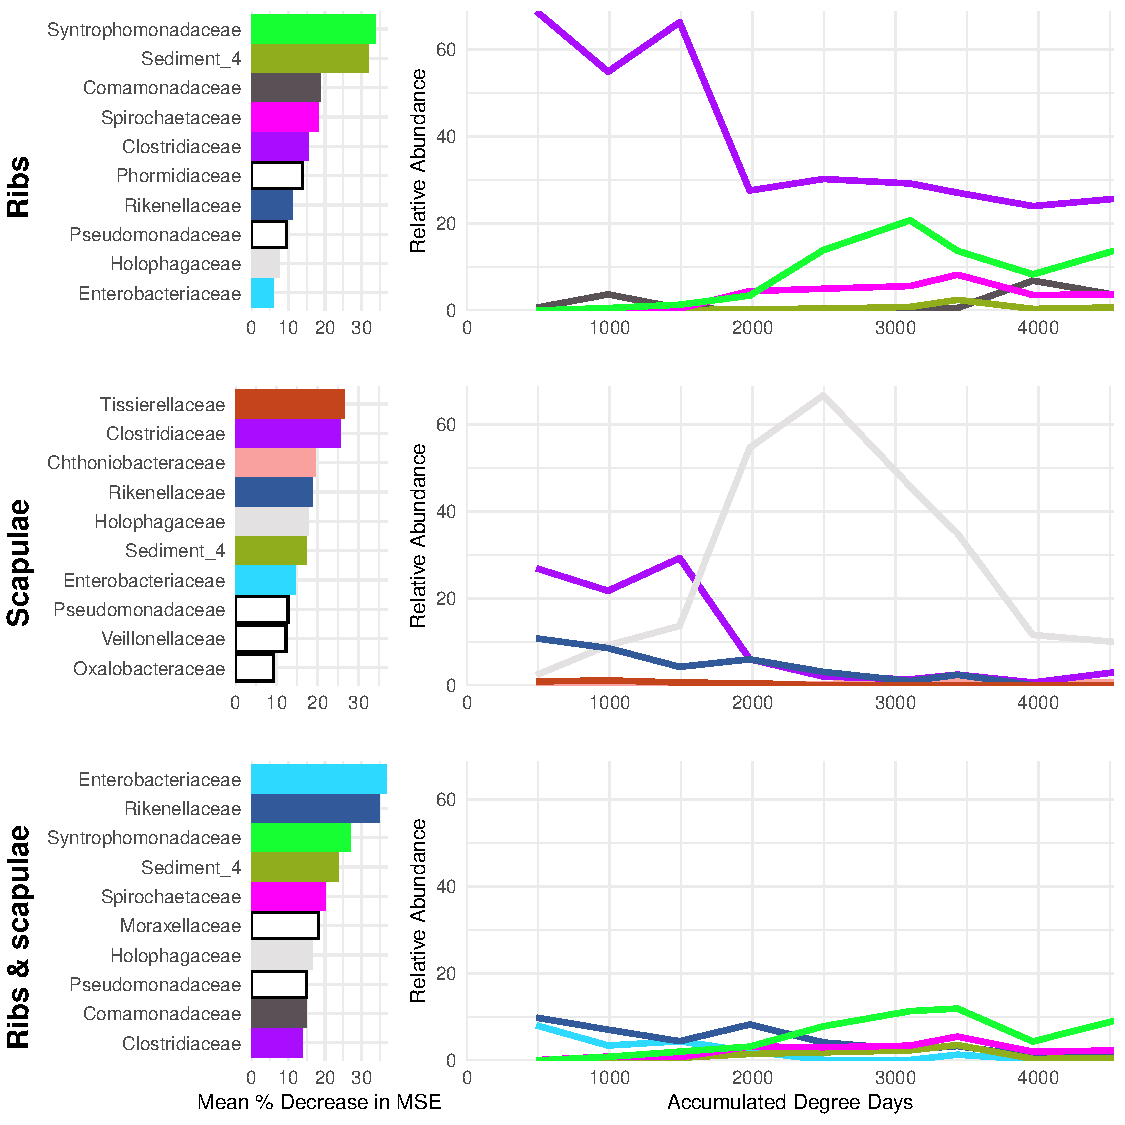
\includegraphics[height=2.85in]
        {w_swabs/bacteria/use_families/hl_combined_family_no_baseline_6panels}
    \end{figure}
  \end{center}

\end{frame}



\begin{frame}{Scatterplots of influential taxa (omitting ADD 0)}

  \begin{center}
    \begin{figure}
      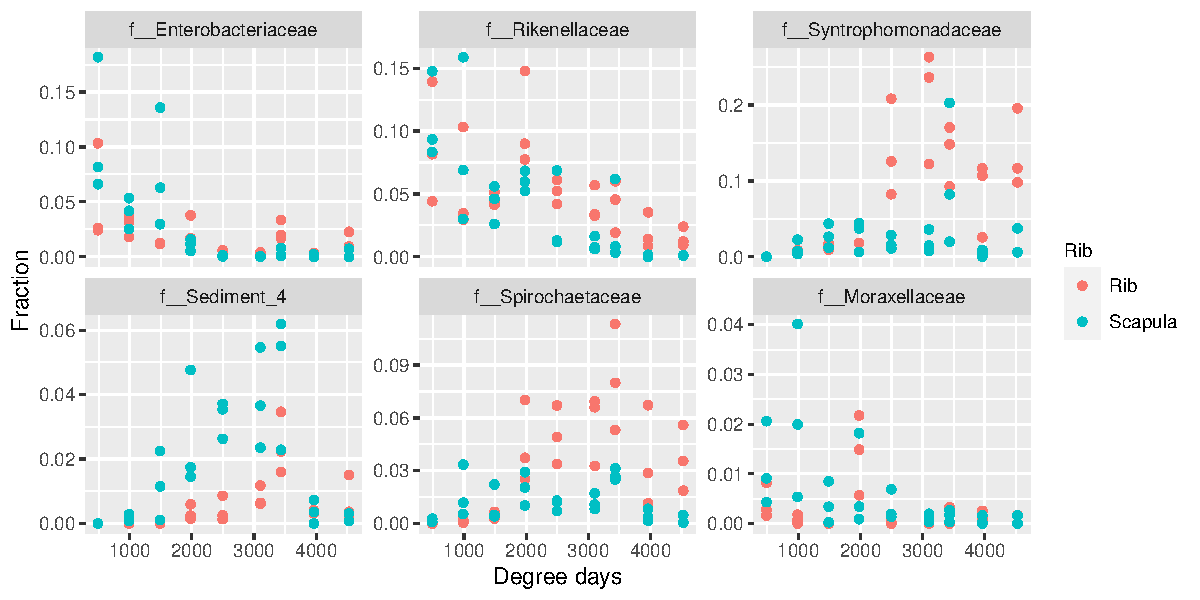
\includegraphics[height=2.1in]
        {w_swabs/bacteria/use_families/both_ribs_scapulae/no_baseline/infl_combined_swab_no_baseline_family_scatter}
    \end{figure}
  \end{center}

  \vspace{0.15in}

  \footnotesize{ \noindent These are the top 6 most influential taxa for the
    combined rib/scapula model.  The scatterplots for Syntrophomonadaceae,
    Sediment\_4, and Spirochaetaceae show differing patterns for ribs and
    scapula.
    }

\end{frame}



\begin{frame}{Pred.\ vs. actual ADD for swabs (omitting ADD 0)}

  \begin{center}
    \begin{figure}
      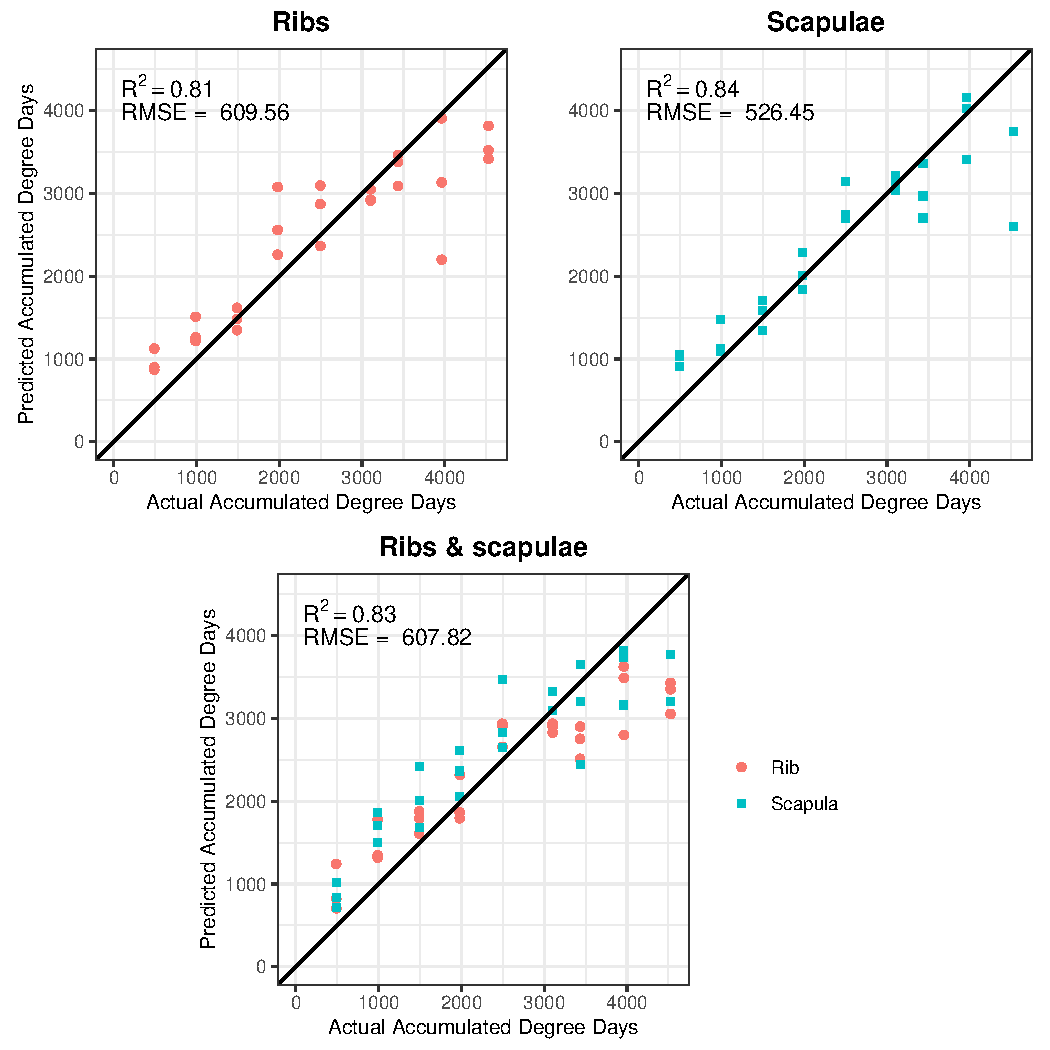
\includegraphics[height=3.1in]
        {w_swabs/bacteria/use_families/hl_combined_family_no_baseline_predicted_vs_actual_ADD}
    \end{figure}
  \end{center}
    
\end{frame}



\begin{frame}{Further comments (omitting ADD 0)}
  
  \begin{itemize}
    \item The following influential taxa in the scapula model were not included
    in the combined rib/scapula model:\\
    Tissierellaceae, Chthoniobacteraceae, Oxalobacteraceae\\
    The first 2 were in the top 5 most influential taxa for the scapula-only
    model, which may be another factor in explaining the oddities of model
    performance in this case.
    \item The following taxa were in the "top 10" influential taxa for all
    three models:\\
    Enterobacteriaceae, Rikenellaceae, Sediment\_4, Holophagaceae,
    Pseudomonadaceae, Clostridiaceae
    
  \end{itemize}

\end{frame}
% %%%%%%%%%%%%%%%%%%%%%%%%%%%%%%%%%%%



% %%%%%%%%%%%%%%%%%%%%%%%%%%%%%%%%%%%
\subsection{Including baseline observations (with ADD 0)}

\begin{frame}{Comparison of rib, scapula, and combined models (swabs, using ADD 0)}

  \begin{tabular}{lrrrr}
    Type & \# samples & \# taxa & RMSE & Expl.\ variation\\ \hline
    Ribs & 30 & 21 & 582.3 & 83.6\% \\
    Scapulae & 28 & 37 & 588.2 & 81.3\% \\
    Combined & 58 & 17 & 623.2 & 80.2\%
  \end{tabular}

  \vspace{0.2in}

  \footnotesize{
    \noindent Again, the combined model doesn't improve things here.  This time,
    the rib-only model in the best fit.\\
    }
\end{frame}



\begin{frame}{Influential taxa for swabs (using ADD 0)}

  \begin{center}
    \begin{figure}
      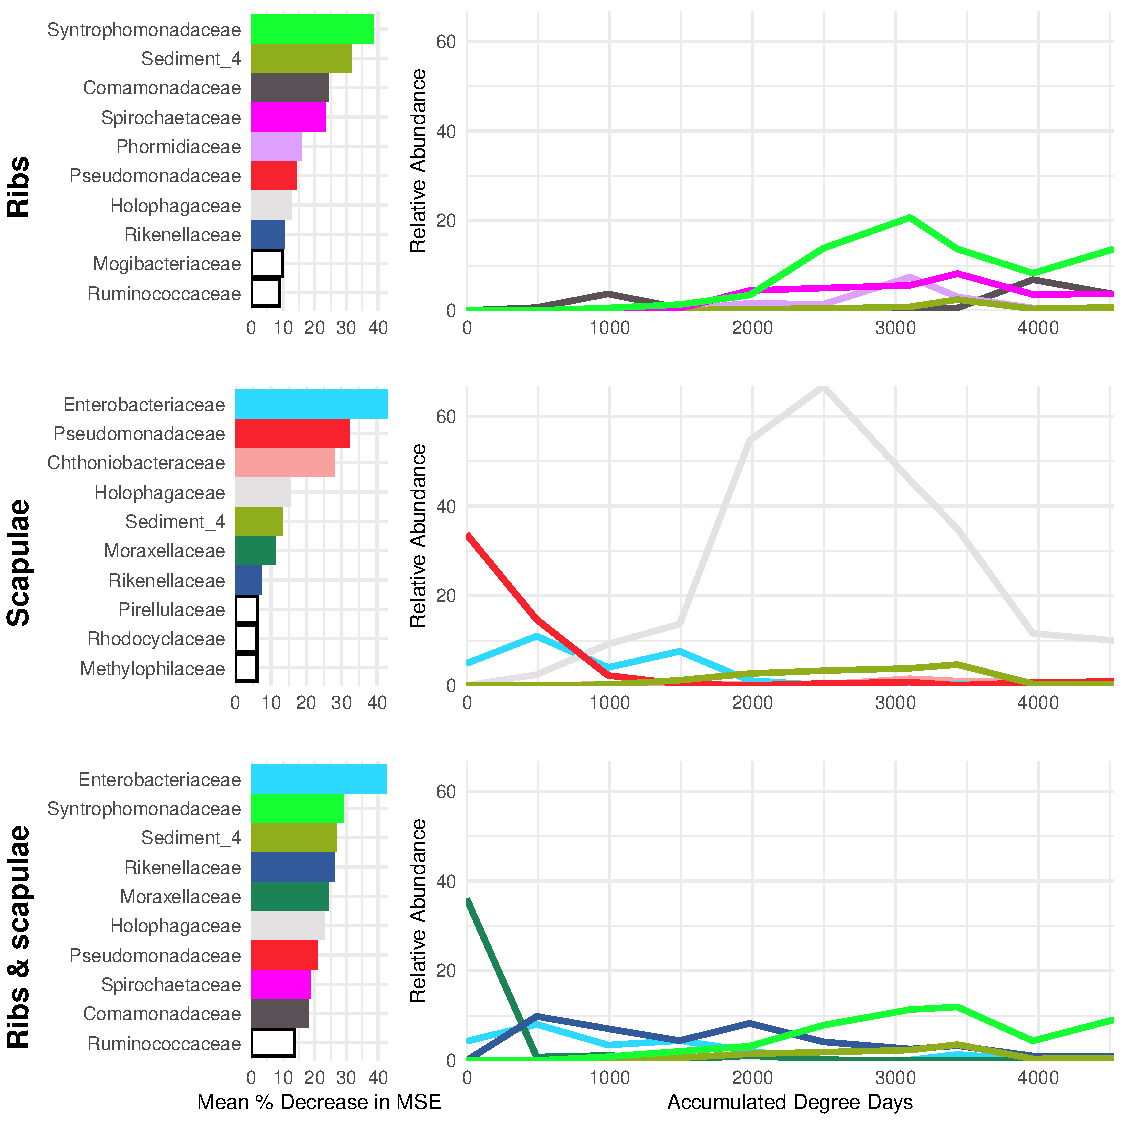
\includegraphics[height=2.85in]
        {w_swabs/bacteria/use_families/hl_combined_family_w_baseline_6panels}
    \end{figure}
  \end{center}

\end{frame}



\begin{frame}{Scatterplots of influential taxa (using ADD 0)}

  \begin{center}
    \begin{figure}
      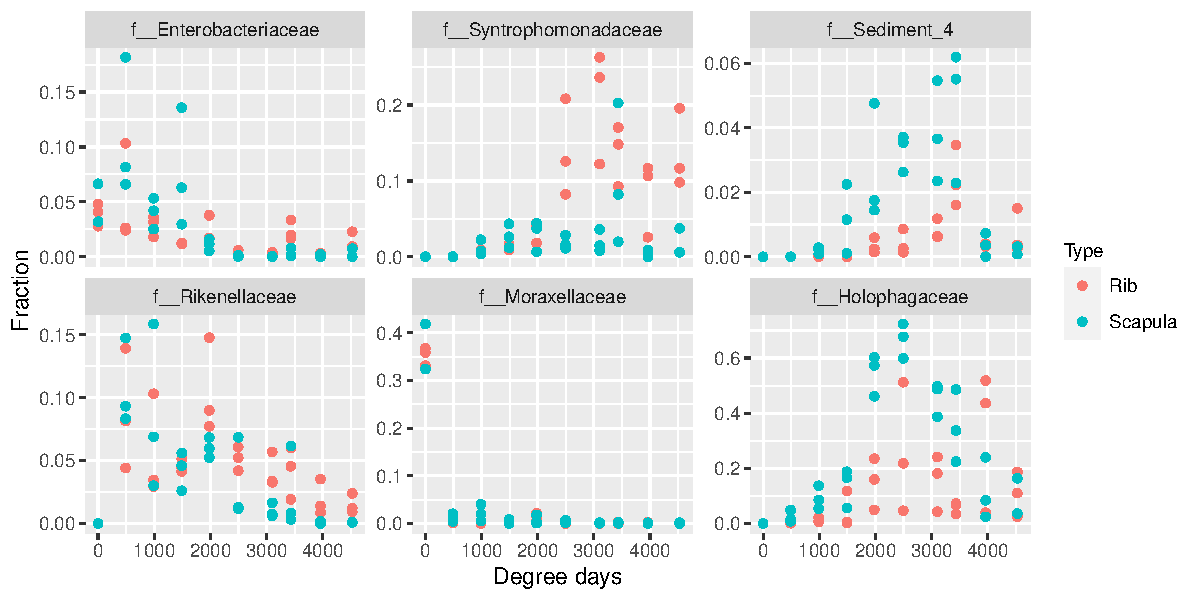
\includegraphics[height=2.1in]
        {w_swabs/bacteria/use_families/both_ribs_scapulae/w_baseline/infl_combined_swab_w_baseline_family_scatter}
    \end{figure}
  \end{center}

  \vspace{0.15in}

  \footnotesize{ \noindent These are the top 6 most influential taxa for the
    combined rib/scapula model.  The scatterplots for Syntrophomonadaceae,
    Sediment\_4, and Holophagaceae show differing patterns for ribs and
    scapula.
    }

\end{frame}



\begin{frame}{Pred.\ vs. actual ADD for swabs (using ADD 0)}

  \begin{center}
    \begin{figure}
      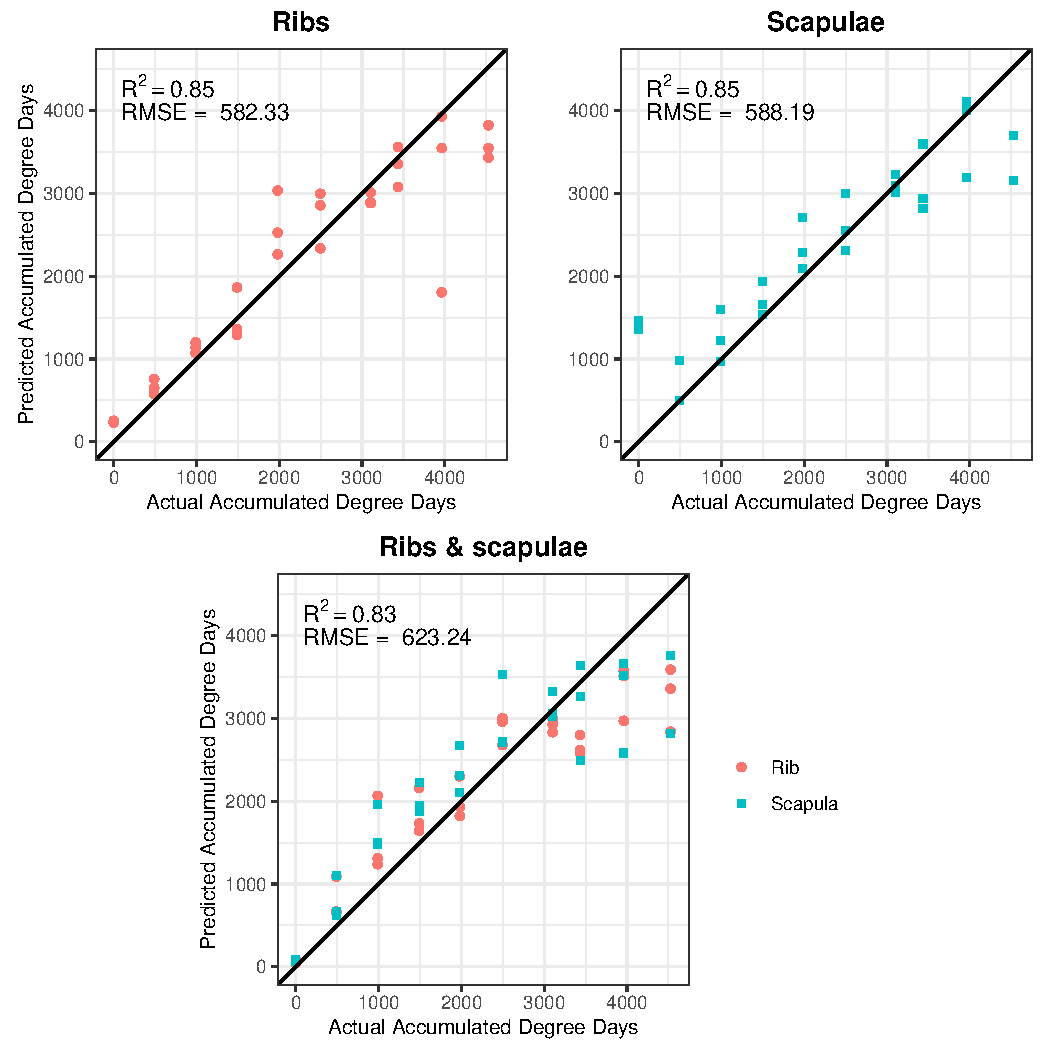
\includegraphics[height=3.1in]
        {w_swabs/bacteria/use_families/hl_combined_family_w_baseline_predicted_vs_actual_ADD}
    \end{figure}
  \end{center}
    
\end{frame}



\begin{frame}{Further comments (using ADD 0)}
  
  \begin{itemize}
    \item The following influential taxa in the scapula model were not included
    in the combined rib/scapula model:\\
    Chthoniobacteraceae, Pirellulaceae, Methylophilaceae
    \item The following taxa were in the "top 10" influential taxa for all
    three models:\\
    Sediment\_4, Rikenellaceae, Holophagaceae, Pseudomonadaceae
  \end{itemize}

\end{frame}
%% %%%%%%%%%%%%%%%%%%%%%%%%%%%%%%%%%%%%%%%%%%%%%%%%%%%%%%%%%%





%% %%%%%%%%%%%%%%%%%%%%%%%%%%%%%%%%%%%%%%%%%%%%%%%%%%%%%%%%%%
\section{Using bones}


% %%%%%%%%%%%%%%%%%%%%%%%%%%%%%%%%%%%
\subsection{Omiting baseline observations}

\begin{frame}{Comparison of rib, scapula, and combined models (bones, omitting ADD 0)}

  \begin{tabular}{lrrrr}
    Type & \# samples & \# taxa & RMSE & Expl.\ variation\\ \hline
    Ribs & 77 & 24 & 540.2 & 87.6\% \\
    Scapulae & 87 & 34 & 331.0 & 95.2\% \\
    Combined & 164 & 23 & 541.0 & 87.4\%
  \end{tabular}

  \vspace{0.2in}

  \footnotesize{
    \noindent The scapulae model performs notably better than the other two.
    }

\end{frame}



\begin{frame}{Influential taxa for swabs (omitting ADD 0)}

  \begin{center}
    \begin{figure}
      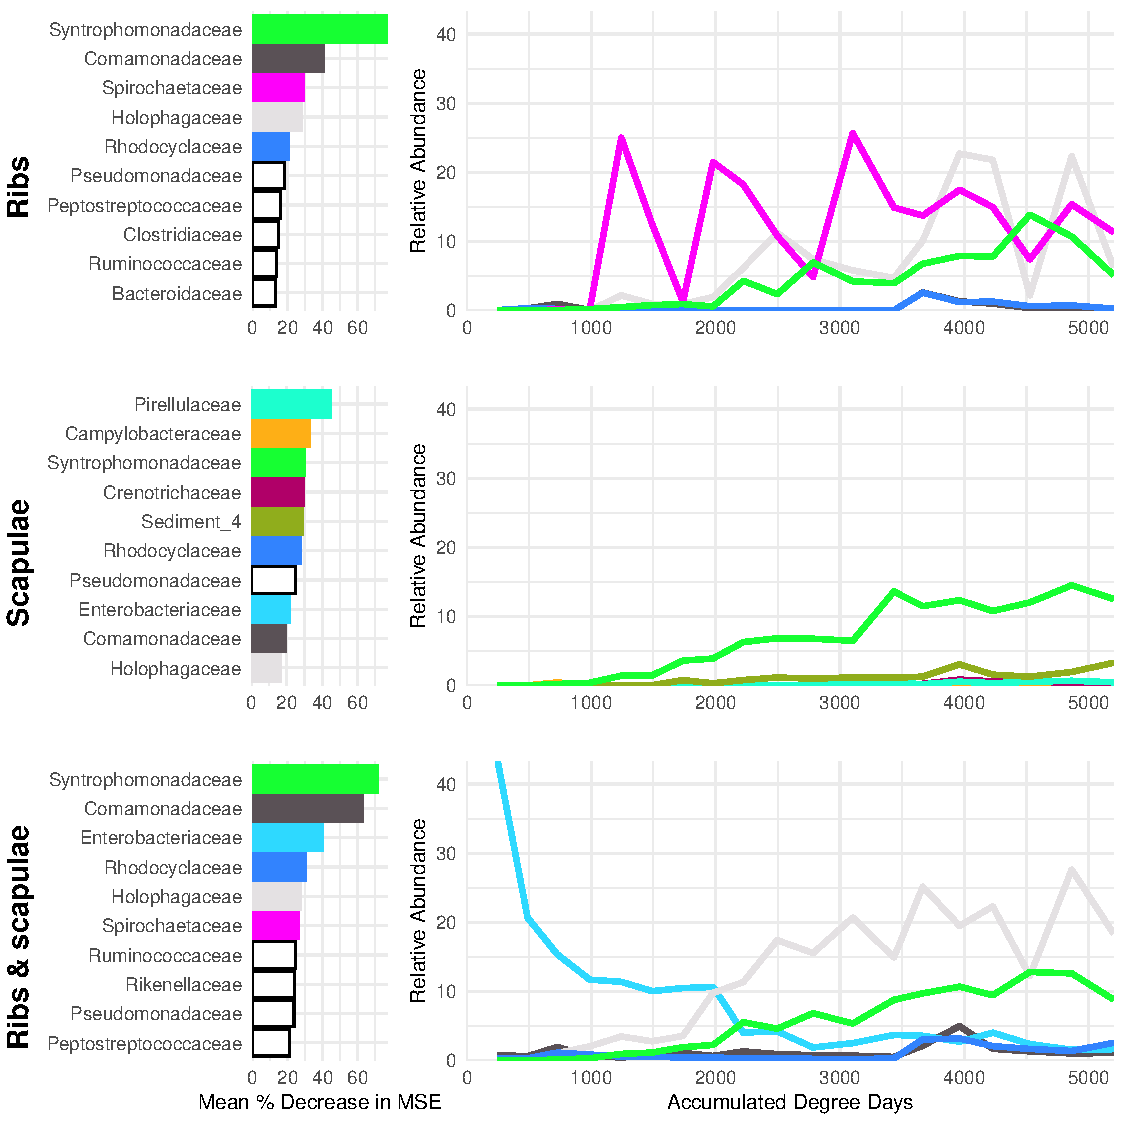
\includegraphics[height=2.85in]
        {w_bones/bacteria/use_families/hl_combined_family_no_baseline_6panels}
    \end{figure}
  \end{center}

\end{frame}



\begin{frame}{Scatterplots of influential taxa (omitting ADD 0)}

  \begin{center}
    \begin{figure}
      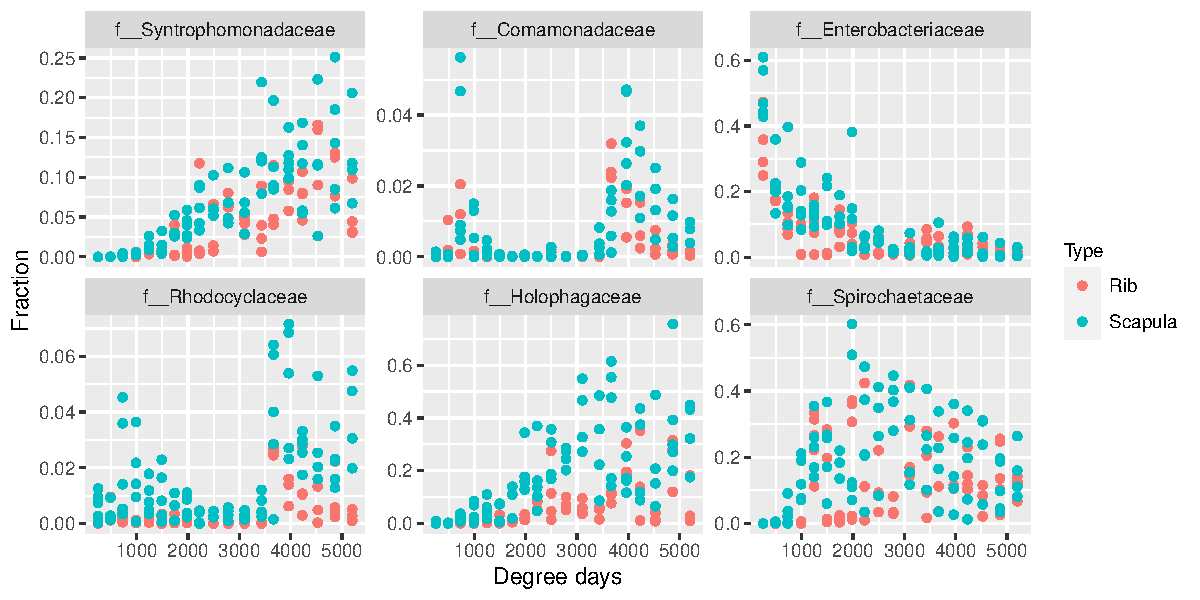
\includegraphics[height=2.1in]
        {w_bones/bacteria/use_families/both_ribs_scapulae/no_baseline/infl_combined_bone_no_baseline_family_scatter}
    \end{figure}
  \end{center}

  \vspace{0.1in}

  \footnotesize{ \noindent These are the top 6 most influential taxa for the
    combined rib/scapula model.  The scatterplots for Syntrophomonadaceae,
    Rhodocyclaceae, and Holophagaceae show that prevalences on scapulae tend to
    be higher.
    }

\end{frame}



\begin{frame}{Pred.\ vs. actual ADD for bones (omitting ADD 0)}

  \begin{center}
    \begin{figure}
      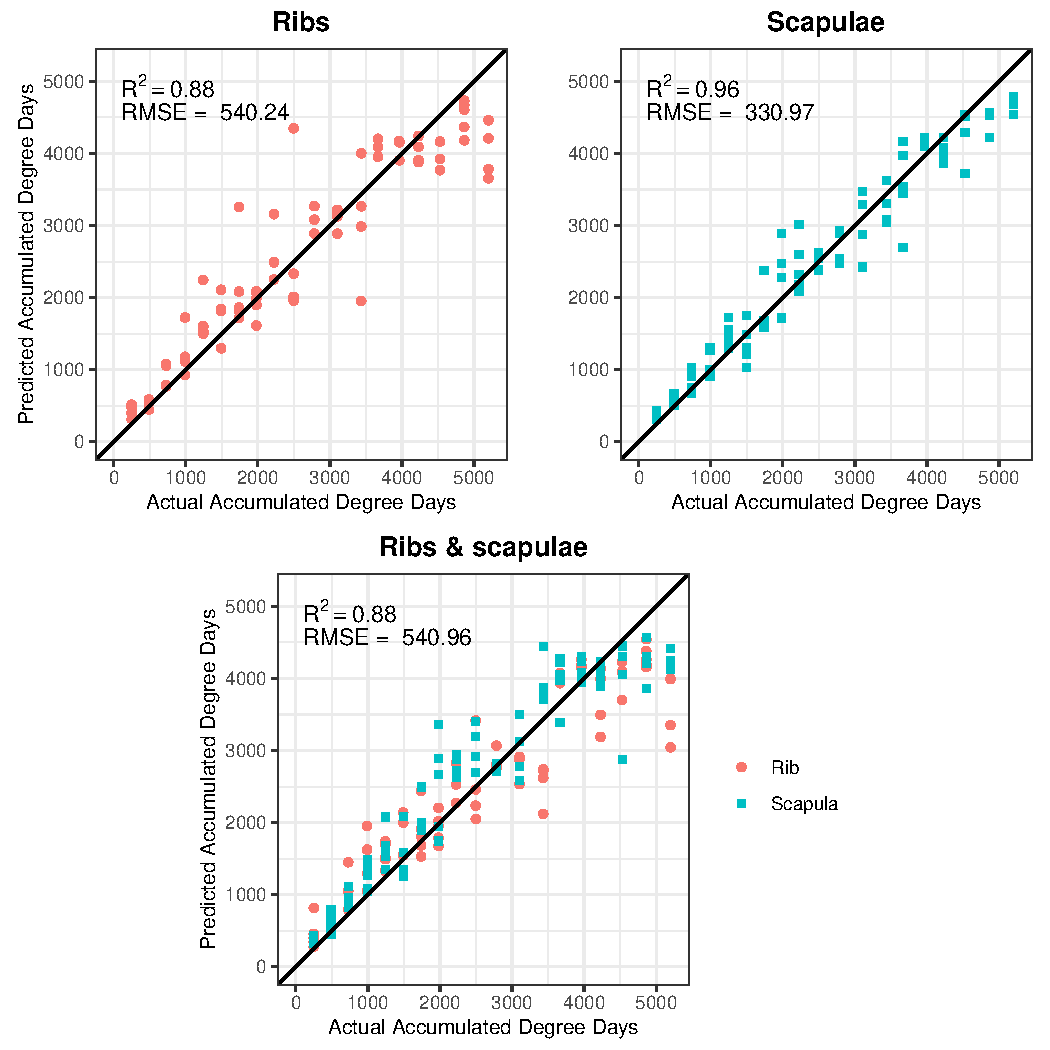
\includegraphics[height=3.1in]
        {w_bones/bacteria/use_families/hl_combined_family_no_baseline_predicted_vs_actual_ADD}
    \end{figure}
  \end{center}
    
\end{frame}




\begin{frame}{Further comments (omitting ADD 0)}
  
  \begin{itemize}
    \item The following taxa were in the "top 10" influential taxa for all
    three models:\\
    Syntrophomonadaceae, Comamonadaceae, Rhodocyclaceae, Holophagaceae,
    Pseudomonadaceae
    \item The following influential taxa in the scapula model were not included
    in the combined rib/scapula model:\\
    Pirellulaceae, Campylobacteraceae, Crenotrichaceae, Sediment\_4
    \item All four of the above taxa are in the top 5 most influential taxa for
    the scapula-only model.  (See graph on next slide.)
    
  \end{itemize}

\end{frame}



\begin{frame}{Scatterplots of influential taxa for scapula-only model}

  \begin{center}
    \begin{figure}
      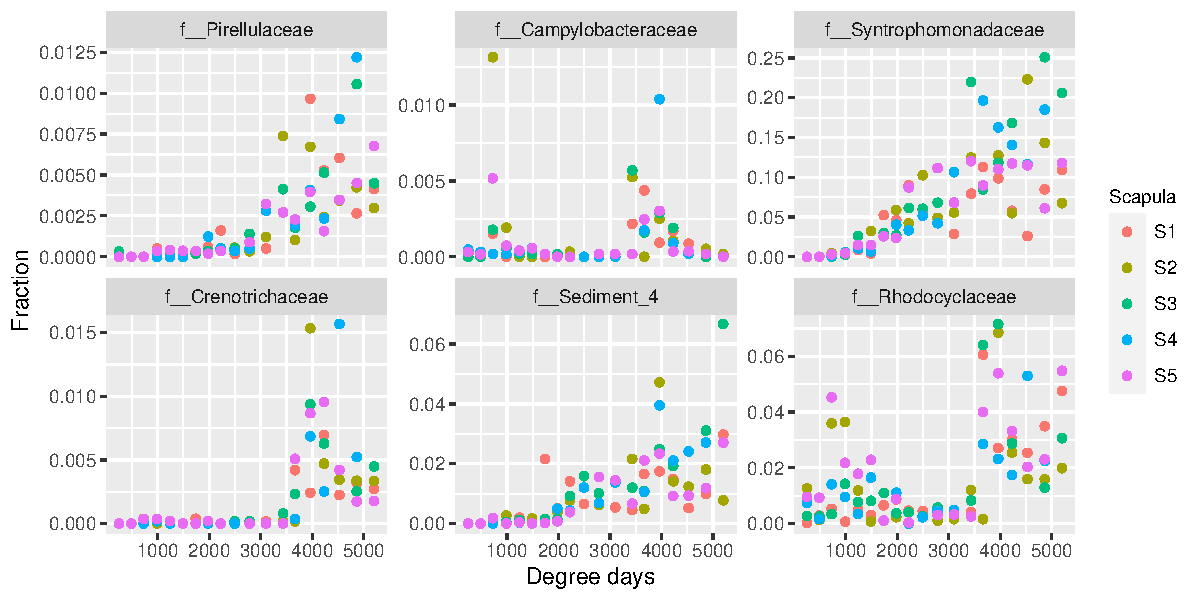
\includegraphics[height=2.1in]
        {w_bones/bacteria/use_families/w_scapulae/no_baseline/infl_scapula_family_no_baseline_scatter}
    \end{figure}
  \end{center}

  \vspace{-0.05in}

  \footnotesize{ \noindent These are the top 6 most influential taxa for the
    \textbf{scapula-only} model.  Look particularly at Pirellulaceae,
    Campylobacteraceae, Crenotrichaceae, and Sediment\_4.  Even though their
    prevalences are very low, they have definite patterns that seem to be
    strengthening the scapula-only model. However, their prevalences in rib data
    are too low to be included in the combined rib/scapula model.
    }

\end{frame}

% %%%%%%%%%%%%%%%%%%%%%%%%%%%%%%%%%%%




% %%%%%%%%%%%%%%%%%%%%%%%%%%%%%%%%%%%
\subsection{Including baseline observations (with ADD 0)}

\begin{frame}{Comparison of rib, scapula, and combined models (bones, using ADD 0)}

  \begin{tabular}{lrrrr}
    Type & \# samples & \# taxa & RMSE & Expl.\ variation\\ \hline
    Ribs & 82 & 24 & 524.0 & 89.3\% \\
    Scapulae & 89 & 34 & 334.1 & 95.3\% \\
    Combined & 171 & 23 & 530.0 & 88.7\%
  \end{tabular}
  
  \vspace{0.2in}

  \footnotesize{ \noindent As we might expect, the addition of the baseline
    samples doesn't change the fact that the scapula-only model performs better
    than the other two. }

\end{frame}



\begin{frame}{Influential taxa for bones (using ADD 0)}

  \begin{center}
    \begin{figure}
      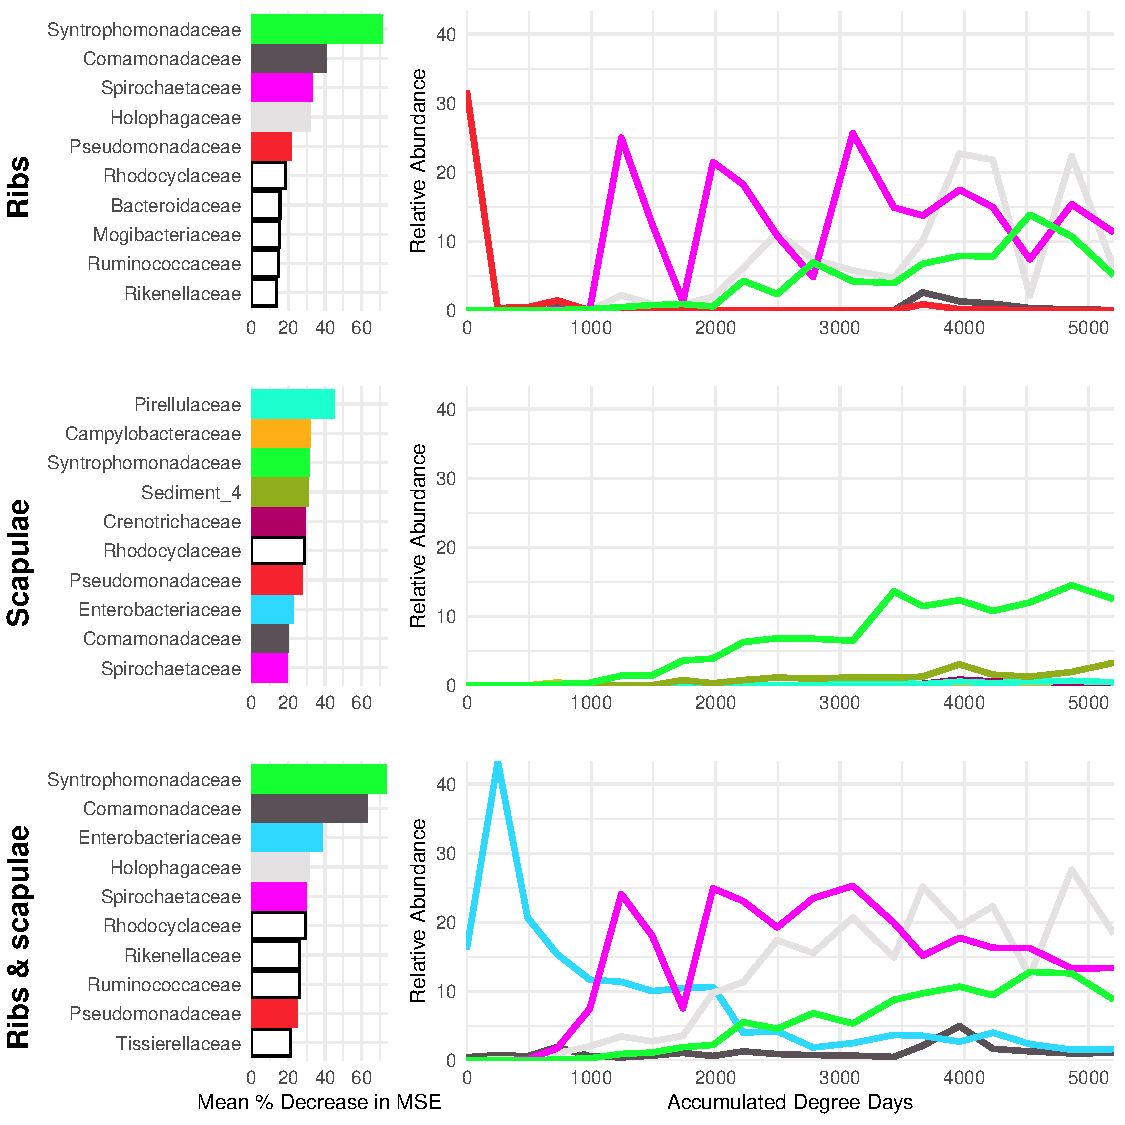
\includegraphics[height=2.85in]
        {w_bones/bacteria/use_families/hl_combined_family_w_baseline_6panels}
    \end{figure}
  \end{center}

\end{frame}



\begin{frame}{Pred.\ vs. actual ADD for bones (using ADD 0)}

  \begin{center}
    \begin{figure}
      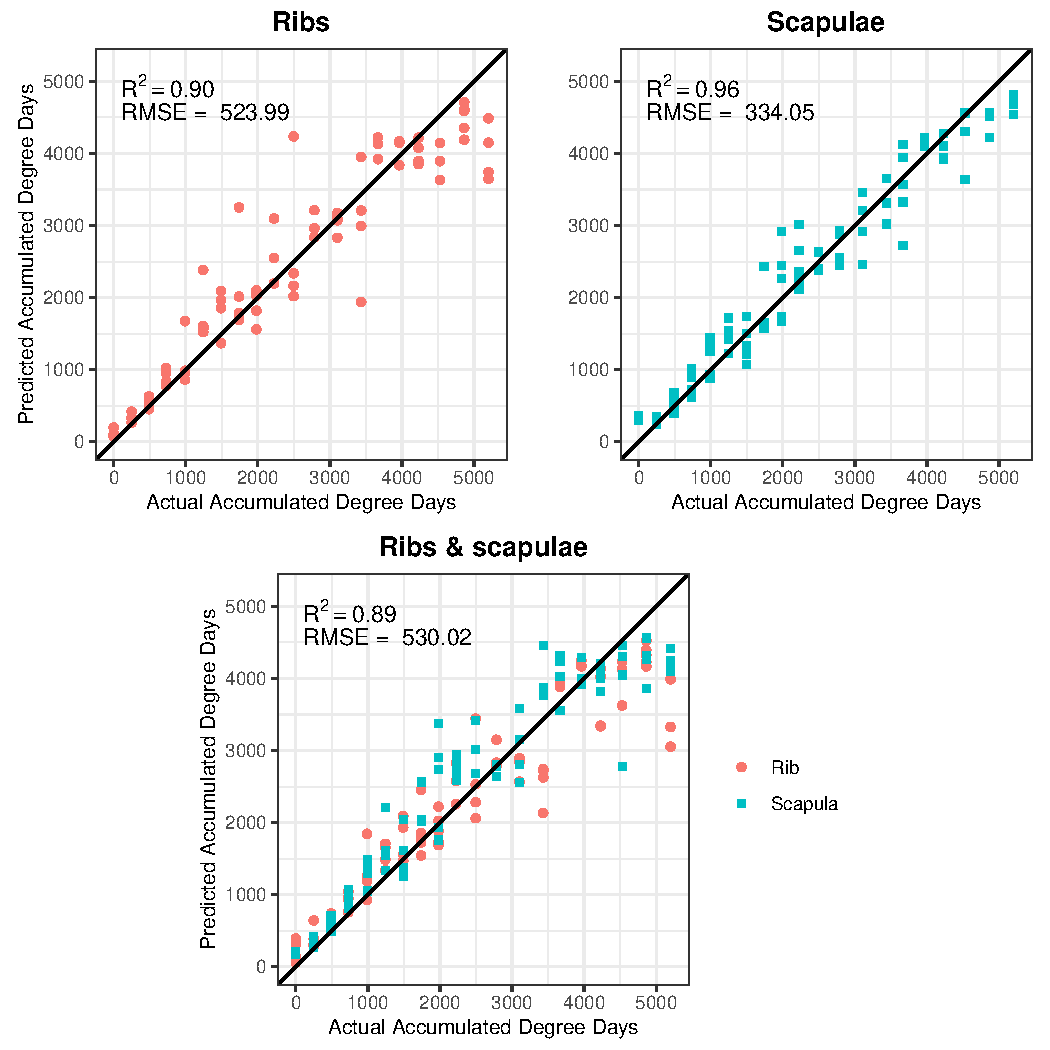
\includegraphics[height=3.1in]
        {w_bones/bacteria/use_families/hl_combined_family_w_baseline_predicted_vs_actual_ADD}
    \end{figure}
  \end{center}
    
\end{frame}



\begin{frame}{Further comments (using ADD 0)}
  
  \begin{itemize}
    \item The following taxa were in the "top 10" influential taxa for all
    three models:\\
    Syntrophomonadaceae, Comamonadaceae, Spirochaetaceae, Rhodocyclaceae, 
    Pseudomonadaceae
    \item As was the case in the bone models which didn't include baseline
    samples, the following influential taxa in the scapula model were not
    included in the combined rib/scapula model:\\
    Pirellulaceae, Campylobacteraceae, Sediment\_4, Crenotrichaceae
    \item Also as before, all four of the above taxa are in the top 5 most
    influential taxa for the scapula-only model.
    
  \end{itemize}

\end{frame}

\end{document}
